\documentclass[11pt]{article}
\usepackage[utf8]{inputenc}
\usepackage[english]{babel}
\usepackage{bilal2vec}
\usepackage{minted}

\title{CO 487 - Assignment 2}
\author{Bilal Khan (b54khan)\\
\href{mailto:bilal.khan@student.uwaterloo.ca}{bilal.khan@student.uwaterloo.ca}}
\date{\today}

\begin{document}

\maketitle

\tableofcontents

\section{1}

This problem uses the simplified cipher described in Section 2 of “A Tutorial on Linear and Differential Cryptanalysis” by Howard M. Heys, available at \url{http://www.engr.mun.ca/~howard/Research/Papers/ldc_tutorial.html}
We refer to this cipher as the “Heys cipher”. For the purposes of this problem, each student has a fixed, unknown 80-bit key.
You will be carrying out a known-plaintext attack against the Heys cipher using linear cryptanalysis, using a set of 20,000 distinct random plaintext-ciphertext pairs.
You can download your plaintexts and ciphertexts at the following addresses:
\url{https://www.math.uwaterloo.ca/~dstebila/as/as.cgi/download/co487_f24/a2q1plaintexts.txt}
and
\url{https://www.math.uwaterloo.ca/~dstebila/as/as.cgi/download/co487_f24/a2q1ciphertexts.txt}
The format of the files is that the nth line of the ciphertext file equals the encryption of the nth line of the plaintext file under your secret key.
For the programming aspects of questions 1.a.i, 1.b, and 1.d.ii, you may work with a partner to do the programming and you may submit the same computer program source code, but you must submit your own write-up and explanations for the non-programming parts of those questions.
Please indicate in your submission who you worked with.

\subsection{a}

Using the linear approximation $U_{4,6} \oplus U_{4,8} \oplus U_{4,14} \oplus U_{4,16} \oplus P_{5} \oplus P_{7} \oplus P_{8} \approx 0$, Carol guesses that the target partial subkey $[K_{5,5}, K_{5,6}, K_{5,7}, K_{5,8}, K_{5,13}, K_{5,14}, K_{5,15}, K_{5,16}]$ has the value $[0, 1, 1, 1, 0, 1, 1, 0]$. Note that Carol's guess is not necessarily correct! Do one of the following:

i. Determine the magnitude of the bias for this partial subkey value over your twenty thousand plaintext/ciphertext pairs, using a computer program, and provide the source code for your program, or:

ii. Determine the magnitude of the bias for this partial subkey value over your first ten plaintext/ciphertext pairs, without using a computer program, and show your work.

The magnitude of the bias is: $0.005049999999999999$

\begin{minted}{python}
import numpy as np
from tqdm import tqdm

s_box = np.array([14, 4, 13, 1, 2, 15, 11, 8, 3, 10, 6, 12, 5, 9, 0, 7])

s_box_inv = np.zeros(16, dtype=np.int32)
for i in range(16):
    s_box_inv[s_box[i]] = i


def read_file(file_path):
    with open(file_path, 'r') as file:
        lines = [line.strip() for line in file]

    blocks = []
    for line in lines:
        blocks.append([int(line[i:i + 4], 2) for i in range(0, 16, 4)])

    return np.array(blocks)


def calculate_bias(plaintexts, ciphertexts, key_guess):
    count = 0
    for plaintext, ciphertext in zip(plaintexts, ciphertexts):
        U = calculate_U_values(ciphertext, key_guess)
        P = calculate_P_values(plaintext)

        linear_approximation = (U[5] ^ U[7] ^ U[13] ^ U[15] ^ P[4] ^ P[6] ^
                                P[7])

        if linear_approximation == 0:
            count += 1

    bias = abs(count / len(plaintexts) - 0.5)
    return bias


def calculate_U_values(ciphertext, key_guess):
    U_blocks = [None] * 4
    for i in range(4):
        U_blocks[i] = s_box_inv[np.bitwise_xor(ciphertext[i], key_guess[i])]

    U = np.zeros(16, dtype=np.int32)
    for i in range(16):
        U[i] = U_blocks[i // 4] >> (3 - i % 4) & 1

    return U


def calculate_P_values(plaintext):
    P = np.zeros(16, dtype=np.int32)
    for i in range(16):
        P[i] = int(plaintext[i // 4] >> (3 - i % 4) & 1)
    return P


plaintexts = read_file('./a2q1plaintexts.txt')
ciphertexts = read_file('./a2q1ciphertexts.txt')


def calculate_key(key_guess):
    binary_to_decimal = np.array([2**3, 2**2, 2**1, 2**0])
    blocks = key_guess.reshape(4, 4)
    blocks_decimal = np.dot(blocks, binary_to_decimal)
    return blocks_decimal


guess = np.zeros(16, dtype=np.int32)
guess[4] = 0
guess[5] = 1
guess[6] = 1
guess[7] = 1
guess[12] = 0
guess[13] = 1
guess[14] = 1
guess[15] = 0

guess_decimal = calculate_key(guess)

bias = calculate_bias(plaintexts, ciphertexts, guess_decimal)
print(f"Bias: {bias}")
\end{minted}

\subsection{b}

Find the value of the partial subkey $[K_{5,5}, K_{5,6}, K_{5,7}, K_{5,8}, K_{5,13}, K_{5,14}, K_{5,15}, K_{5,16}]$ for your key, by calculating the target partial subkey which yields the largest magnitude of bias over your 20,000 plaintext/ciphertext pairs. You will almost certainly need a computer program for this task; provide the source listing for any computer code that you or your collaborators write.

Best Subkey: $[0 0 0 0 1 1 0 0 0 0 0 0 1 0 0 0]$
Max Bias: $0.032200000000000006$

\begin{minted}{python}
def find_best_key(plaintexts, ciphertexts):
    max_bias = 0
    best_subkey = None

    for subkey in tqdm(range(256)):
        guess = np.zeros(16, dtype=np.int32)
        guess[4] = (subkey >> 7) & 1
        guess[5] = (subkey >> 6) & 1
        guess[6] = (subkey >> 5) & 1
        guess[7] = (subkey >> 4) & 1
        guess[12] = (subkey >> 3) & 1
        guess[13] = (subkey >> 2) & 1
        guess[14] = (subkey >> 1) & 1
        guess[15] = subkey & 1

        guess_decimal = calculate_key(guess)

        bias = calculate_bias(plaintexts, ciphertexts, guess_decimal)

        if bias > max_bias:
            max_bias = bias
            best_subkey = guess.copy()

    return best_subkey, max_bias


best_subkey, max_bias = find_best_key(plaintexts, ciphertexts)
print(f"Best Subkey: {best_subkey}")
print(f"Max Bias: {max_bias}")
\end{minted}

\subsection{c}

By using Table 4 in the tutorial, compute the bias in each of the following individual S-box linear approximations:

\begin{align*}
    S_{11} : X_{1} \oplus X_{4} \approx Y_{1} \\
    S_{13} : X_{1} \oplus X_{4} \approx Y_{1} \\
    S_{21} : X_{1} \oplus X_{3} \approx Y_{2} \\
    S_{32} : X_{1} \approx Y_{1} \oplus Y_{2} \oplus Y_{3} \oplus Y_{4}   
\end{align*}
Then, combine these to find a linear approximation of the first three rounds of the Heys cipher,
and calculate the theoretical magnitude of its bias.

$b_1, b_2, b_3, b_4 = 2^3, 2^2, 2^1, 2^0 = 8, 4, 2, 1$

\begin{align*}
    S_{11} : X_{1} \oplus X_{4} \approx Y_{1}, \text{probability = $4/16$, bias $= -1/4$} \\
    S_{13} : X_{1} \oplus X_{4} \approx Y_{1}, \text{probability = $4/16$, bias $= -1/4$} \\
    S_{21} : X_{1} \oplus X_{3} \approx Y_{2}, \text{probability = $4/16$, bias $= -1/4$} \\
    S_{32} : X_{1} \approx Y_{1} \oplus Y_{2} \oplus Y_{3} \oplus Y_{4}, \text{probability = 2/16$$, bias $= -6/16$}
\end{align*}

\begin{align*}
    V_{1,1} &= U_{1,1} \oplus U_{1,4} \\
            &= (P_1 \oplus K_{1,1}) \oplus (P_4 \oplus K_{1,4}) \\
    V_{1,9} &= U_{1,9} \oplus U_{1,12} \\
            &= (P_9 \oplus K_{1,9}) \oplus (P_{12} \oplus K_{1,12}) \\
    V_{2,2} &= U_{2,1} \oplus U_{2,3} \\
            &= (V_{1,1} \oplus K_{2,1}) \oplus (V_{1,9} \oplus K_{2,9}) \\
    V_{3,5} \oplus V_{3,6} \oplus V_{3,7} \oplus V_{3,8} &= U_{2,5} \\
            &= (V_{2,2} \oplus K_{3,5}) \\
    0 &\approx V_{3,5} \oplus V_{3,6} \oplus V_{3,7} \oplus V_{3,8} \oplus P_1 \oplus P_4 \oplus P_9 \oplus P_{12} \oplus K_{1,1} \oplus K_{1,4} \\
    & \oplus K_{1,9} \oplus K_{1,12} \oplus K_{2,1} \oplus K_{2,9} \oplus K_{3,5} \\
    U_{4,2} &= V_{3,5} \oplus K_{4,2} \\
    U_{4,6} &= V_{3,6} \oplus K_{4,6} \\
    U_{4,10}&= V_{3,7} \oplus K_{4,10} \\
    U_{4,14}&= V_{3,8} \oplus K_{4,14} \\
    0 &\approx U_{4,2} \oplus U_{4,6} \oplus U_{4,10} \oplus U_{4,14} \oplus P_1 \oplus P_4 \oplus P_9 \oplus P_{12} \\
    &\oplus K_{1,1} \oplus K_{1,4} \oplus K_{1,9} \oplus K_{1,12} \oplus K_{2,1} \oplus K_{2,9} \oplus K_{3,5}\\
    &\oplus K_{4,2} \oplus K_{4,6} \oplus K_{4,10} \oplus K_{4,14}
\end{align*}

\begin{align*}
    U_{4,2} \oplus U_{4,6} \oplus U_{4,10} \oplus U_{4,14} \oplus P_1 \oplus P_4 \oplus P_9 \oplus P_ {12} &\approx 0
\end{align*}

The probability is given by: $1/2 + 2^{4-1} (-1/4) (-1/4) (-1/4) (-6/16) = 0.546875$ and the bias is $0.046875$

\subsection{d}

Do one of the following:

i. Using the linear approximation from part (c), determine the entire subkey $K_5$. You will almost certainly need a computer program for this task; provide the source listing for any computer code that you or your collaborators write, or:

ii. Using the (incorrect) guess $K_5 = [1100011111100110]$ for the fifth subkey, determine the magnitude of the bias of the approximation from part (c) for this subkey over your first ten plaintext/ciphertext pairs, without using a computer program, and show your work.

The Best Subkey: $[0 0 0 0 0 1 0 1 0 0 0 0 1 1 0 1]$
Max Bias: $0.012750000000000039$

\begin{minted}{python}
    import numpy as np
    from tqdm import tqdm
    
    s_box = np.array([14, 4, 13, 1, 2, 15, 11, 8, 3, 10, 6, 12, 5, 9, 0, 7])
    
    s_box_inv = np.zeros(16, dtype=np.int32)
    for i in range(16):
        s_box_inv[s_box[i]] = i
    
    
    def read_file(file_path):
        with open(file_path, 'r') as file:
            lines = [line.strip() for line in file]
    
        blocks = []
        for line in lines:
            blocks.append([int(line[i:i + 4], 2) for i in range(0, 16, 4)])
    
        return np.array(blocks)
    
    
    def calculate_bias(plaintexts, ciphertexts, key_guess):
        count = 0
        for plaintext, ciphertext in zip(plaintexts, ciphertexts):
            U = calculate_U_values(ciphertext, key_guess)
            P = calculate_P_values(plaintext)
    
            #        linear_approximation = (U[5] ^ U[7] ^ U[13] ^ U[15] ^ P[4] ^ P[6] ^
            #                                P[7])
            linear_approximation = (U[0] ^ U[5] ^ U[9] ^ U[13] ^ P[0] ^ P[3] ^
                                    P[8] ^ P[11])
    
            if linear_approximation == 0:
                count += 1
    
        bias = abs(count / len(plaintexts) - 0.5)
        return bias
    
    
    def calculate_U_values(ciphertext, key_guess):
        U_blocks = [None] * 4
        for i in range(4):
            U_blocks[i] = s_box_inv[np.bitwise_xor(ciphertext[i], key_guess[i])]
    
        U = np.zeros(16, dtype=np.int32)
        for i in range(16):
            U[i] = U_blocks[i // 4] >> (3 - i % 4) & 1
    
        return U
    
    
    def calculate_P_values(plaintext):
        P = np.zeros(16, dtype=np.int32)
        for i in range(16):
            P[i] = int(plaintext[i // 4] >> (3 - i % 4) & 1)
        return P
    
    
    plaintexts = read_file('./a2q1plaintexts.txt')
    ciphertexts = read_file('./a2q1ciphertexts.txt')
    
    
    def calculate_key(key_guess):
        binary_to_decimal = np.array([2**3, 2**2, 2**1, 2**0])
        blocks = key_guess.reshape(4, 4)
        blocks_decimal = np.dot(blocks, binary_to_decimal)
        return blocks_decimal
    
    
    guess = np.zeros(16, dtype=np.int32)
    guess[4] = 0
    guess[5] = 1
    guess[6] = 1
    guess[7] = 1
    guess[12] = 0
    guess[13] = 1
    guess[14] = 1
    guess[15] = 0
    
    guess_decimal = calculate_key(guess)
    
    bias = calculate_bias(plaintexts, ciphertexts, guess_decimal)
    print(f"Bias: {bias}")
    
    
    def find_best_key(plaintexts, ciphertexts):
        max_bias = 0
        best_subkey = None
    
        for subkey in tqdm(range(256)):
            guess = np.zeros(16, dtype=np.int32)
            guess[4] = (subkey >> 7) & 1
            guess[5] = (subkey >> 6) & 1
            guess[6] = (subkey >> 5) & 1
            guess[7] = (subkey >> 4) & 1
            guess[12] = (subkey >> 3) & 1
            guess[13] = (subkey >> 2) & 1
            guess[14] = (subkey >> 1) & 1
            guess[15] = subkey & 1
    
            guess_decimal = calculate_key(guess)
    
            bias = calculate_bias(plaintexts, ciphertexts, guess_decimal)
    
            if bias > max_bias:
                max_bias = bias
                best_subkey = guess.copy()
    
        return best_subkey, max_bias
    
    
    best_subkey, max_bias = find_best_key(plaintexts, ciphertexts)
    print(f"Best Subkey: {best_subkey}")
    print(f"Max Bias: {max_bias}")    
\end{minted}

\subsection{e} 

A small amount of extra credit is available if you can determine any additional
key bits.

\newpage

\section{2}

This question is meant to illustrate the importance of proper implementation. The Jupyter notebook Penguins.ipynb (available on LEARN) contains Python implementations of four different block cipher modes of operation: ECB, CBC, OFB, and CTR. Some have been implemented correctly, and some have not. You have also been provided with four encrypted image files, which you can download from LEARN:

• image1.ppm, which was encrypted using ECB mode

• image2.ppm, which was encrypted using CBC mode and the IV specified in the Jupyter notebook

• image3.ppm, which was encrypted using OFB mode and the IV specified in the Jupyter notebook

• image4.ppm, which was encrypted using CTR mode and the IV specified in the Jupyter notebook

Some of the above files are the encryptions of images of penguins, and some are not. By analyzing the encrypted images and the code in Penguins.ipynb that was used to encrypt them, your task is to determine which of the images are penguins, and which are not. For each image/mode, you should explain:

• Whether there is a flaw in the implementation of the mode of operation, and what the flaw is.

• Whether the plaintext image is:

(a) DEFINITELY A PENGUIN

(b) DEFINITELY NOT A PENGUIN

(c) CANNOT BE CERTAIN WHETHER OR NOT IT IS A PENGUIN

Image1/ECB Mode: No flaw, CANNOT BE CERTAIN WHETHER OR NOT IT IS A PENGUIN

Image2/CBC Mode: The key is not used at all, and is instead replaced by $iv + iv$

This means we can use the IV as the key and decrypt the image.

\begin{minted}{diff}
-    iv = AES_encrypt_one_block(iv+iv, x)
+    iv = AES_encrypt_one_block(key, x)
\end{minted}

\begin{minted}{python}
def CBC_mode_decrypt_buggy(key, iv, ciphertext):
    pt = b'' 
    for i in range(0, len(ciphertext), 16):
        ctblock = ciphertext[i:i+16]
        x = AES_decrypt_one_block(iv+iv, ctblock)
        x = bytes(iv[j] ^ x[j] for j in range(16))
        pt += x
        iv = ctblock

    return pt

(header1, header2, header3, image) = read_in_image("a2q2ciphertexts/image2.ppm")
decrypted_image = CBC_mode_decrypt_buggy(None, iv_cbc, image)
write_ppm_file("decrypted_image2.ppm", header1, header2, header3, decrypted_image)
display_image("decrypted_image2.ppm")
\end{minted}

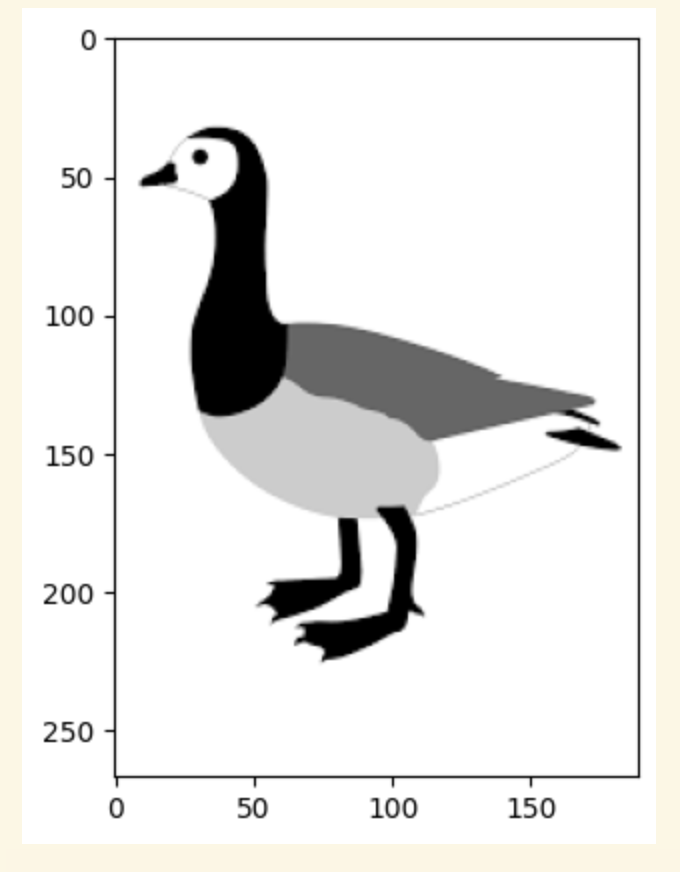
\includegraphics[width=0.5\textwidth]{a2q2_1.png}

Using this code, we can see that the image is of a Goose and not a Penguin. DEFINITELY NOT A PENGUIN

Image3/OFB Mode: No issue, CANNOT BE CERTAIN WHETHER OR NOT IT IS A PENGUIN

Image4/CTR Mode: The counter is never incremented and the IV and counter are added instead of being concatenated. Essentially, this is using a static key thats given by the IV. to encrypt the image.

We can't fully or partially decrypt the image by for example using a known plaintext attack and xor-ing two ciphertexts together to get rid of the keystream since the key is unknown.

However, the property of CTR using the same key (key + the static 0000 counter) means that identical blocks get mapped to identical ciphertext blocks. Given that we use blocks of 16 bytes at a time, we can sometimes see patterns in the ciphertext that correspond to patches of color or structures from the original image. In this case, we can see that the image is of a Penguin just by visualizing the ciphertext image. DEFINITELY A PENGUIN

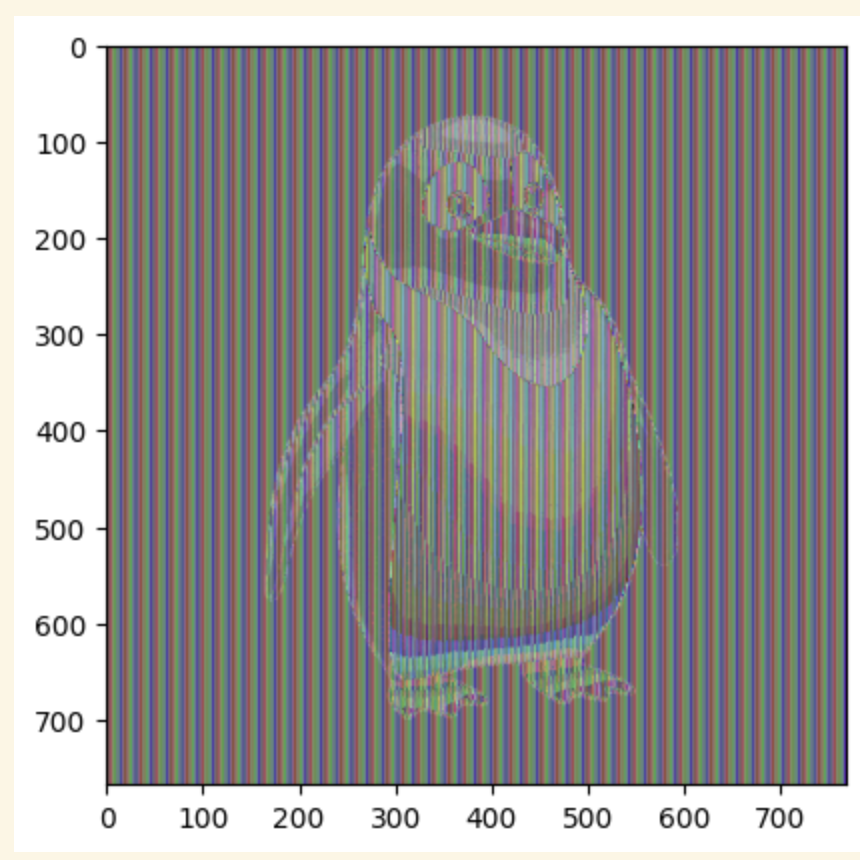
\includegraphics[width=0.5\textwidth]{a2q2_2.png}

In each case, you must fully justify your answer. (Note: “Because it looks like a penguin” is not a fully justified answer. However this doesn’t mean you have to fully decrypt every image.)

\newpage

\section{3}

We generally assume that the adversary does not know the secret key, but does know the initialization vector. Suppose that, for OFB mode, we kept the IV secret as well. Show that this does not make an exhaustive key search any more expensive - in other words, show how to perform a brute-force attack on OFB with an unknown key and an unknown IV. What requirements have you made on the plaintext and ciphertext?

The requirements for an efficient brute-force attack is that we must have a known plaintext-ciphertext pair encrypted under the same key and IV. Given a known plaintext-ciphertext pair $(P, C)$, we can calculate the IV used for a given key in a single step by just running the encryption algorithm in reverse for the zero-th block of the ciphertext. OFB encryption/decryption is defined as:

\begin{align*}
    O_0 &= IV \\
    O_i &= E(K, O_{i-1}) \\
    C_i &= O_i \oplus P_i \\
    P_i &= O_i \oplus C_i
\end{align*}


Encrypting a plaintext into its ciphertext given a key and IV by $C_i = E(K, IV) \oplus P_i$.
Decrypting a ciphertext into its plaintext given a key and IV by $P_i = E(K, IV) \oplus C_i$.

Computing the IV is then simply done by running the encryption function in reverse ($E^{-1}$): $IV = E^{-1}(K, C_0 \oplus P_0)$.

This step is fast and lets us compute the IV for a given key in a single step. We can then brute-force the key in the usual way by trying all keys and checking if the decoded IV lets us decrypt the ciphertext back to the plaintext, the only overhead being that we need to run the ecryption function twice (once backwards for the IV and once forwards to decode the ciphertext) for every key that we try.

\newpage

\section{4}

Trits are similar to bits but have three possible values $\{0, 1, 2\}$ instead of two. As such, they can be seen as elements in $\mathbb{Z}_3$ - integers modulo $3$. They are sometimes used in algorithms where the objects we are working with have three possible states, such as walks on 3-regular graphs. 

For two strings of trits with same length $(t_1, \cdots , t_n)$ and $(t^\prime_1, \cdots , t^\prime_n)$, we can define the subtraction operation as:
n), we can define the subtraction operation as

$$ (t_1, \cdots , t_n) - (t^\prime_1, \cdots , t^\prime_n) := (t_1 - t^\prime_1, \cdots , t_n - t^\prime_n) $$

where each tritwise operation is done modulo $3$.

Let $f : \{0, 1, 2\}^m \rightarrow \{0, 1, 2\}^m$ be a preimage-resistant bijection.

For $x \in \{0, 1, 2\}^{2m}$, write $x = x^\prime || x^{\prime \prime}$ (in other words, split the $2m$-trit string $x$ into two $m$-trit halves: $x^\prime$ and $x^{\prime\prime}$). Define a new hash function $H : \{0, 1, 2\}^{2m} \rightarrow \{0, 1, 2\}^m$ by:

$$ H(x) = f(x^\prime) - f(x^{\prime\prime}) $$

\subsection{a}

For sufficiently large values of $m$ (e.g., $m = 256$), does $H$ have each of the following desired properties for a cryptographic hash function? If yes, justify your answer with a contrapositive argument. If no, justify your answer by showing how to break the property.

i. Preimage resistance

We want to prove that if $f$ is preimage resistant, then $H$ is preimage resistant.

We can prove the contrapositive: if $H$ is not preimage resistant, then $f$ is not preimage resistant.

For a given $y$, we can find $x = x^\prime || x^{\prime\prime}$ such that $H(x) = f(x^\prime) - f(x^{\prime\prime}) \mod 3 = y \mod 3$.

This means that we can now find a preimage for $f$ given our $y$ and the $x^\prime, x^{\prime\prime}$ that we found by inverting $H$.

Rearranging,

\begin{align*}
    f(x^\prime) - f(x^{\prime\prime}) \mod 3 &= y \\
    f(x^\prime) \mod 3 &= y + f(x^{\prime\prime}) \mod 3 \\
    x^\prime &= f^{-1}(y + f(x^{\prime\prime})) \mod 3
\end{align*}

This means that we can find a preimage for $f$ given our $y$ and the $x^\prime, x^{\prime\prime}$ that we found by inverting $H$.

This is a contradiction to the fact that $f$ is preimage resistant, therefore $H$ is preimage resistant.

ii. Second preimage resistance

We want to prove that if $f$ is preimage resistant, then $H$ is second preimage resistant.

We can prove the contrapositive: if $H$ is not second preimage resistant, then $f$ is not preimage resistant.

If $H$ is not second preimage resistant, then there are two inputs $x_1 = x^\prime_1 || x^{\prime\prime}_1$ and $x_2 = x^\prime_2 || x^{\prime\prime}_2$ such that $H(x_1) = H(x_2)$.

Rearranging,

\begin{align*}
    H(x_1) &= H(x_2) \\
    f(x^\prime_1) - f(x^{\prime\prime}_1) &= f(x^\prime_2) - f(x^{\prime\prime}_2) \mod 3 \\
    f(x^\prime_1) &= f(x^{\prime\prime}_1) + (f(x^\prime_2) - f(x^{\prime\prime}_2)) \mod 3 \\
    t &= f(x^\prime_2) - f(x^{\prime\prime}_2) \mod 3 \\
    x^\prime_1 &= f^{-1}(f(x^{\prime\prime}_1) + t) \mod 3
\end{align*}

This means that we can now find a preimage for $f$ given our $x_1, x_2$ and the fact that $H(x_1) = H(x_2)$ from finding a second preimage for $H$.

This is a contradiction to the fact that $f$ is preimage resistant, therefore $H$ is second preimage resistant.

iii. Collision resistance

\subsection{b}

Suppose $m = 128$, so that the input space for H is $\{0, 1, 2\}^256$ and the output space is $\{0, 1, 2\}^128$. If you sample the inputs uniformly at random, what is the expected number of steps before you find a collision in H? It is okay to use an approximation here, as long you state, and justify that approximation.

We can use the birthday paradox for this, $t \approx \sqrt{\pi * N / 2}$, where $N$ is the number of possible values to sample from. Assuming a perfect hash function that uniformly maps $256$ trits to $128$ trits, we have $N = 3^{128}$, and therefore $t \approx \sqrt{\pi * 3^{128} / 2} \approx 4.3 \times10^{30}$ steps before a collision..

\newpage

\section{5}

The sponge construction is a key part in multiple cryptographic schemes, most notably the SHA-3 hash function. The construction has the following properties:

• A message m of length $nl$ is separated into n blocks $(m_1,\cdots,m_n)$ each of length $l$.

• The initialization vector $v$ is of length $l + r$, and is separated into a two potions $v = v_1 || v_2$, where $v_1$ is $l$ bits in length and $v_2$ is $r$ bits in length.

• $\pi : \{0,1\}^{l+r} \rightarrow \{0,1\}^{l+r}$ is a hard-to-invert permutation.

Here is the pseudocode for a sponge construction based on $\pi$ that takes an input message $m$ of length $nl$, and produces an output $g$ of length $sl$.

\begin{minted}{python}
    def H(m):
        h_1 || h_2 = v_1 || v_2
        for i in range(n):
            h_1 = h_1 xor m_i
            h_1 || h_2 = pi(h_1 || h_2)
        for j in range(s):
            g_j = h_1
            h_1 || h_2 = pi(h_1 || h_2)
        return g_1 || g_2 || ... || g_s
\end{minted}

The first loop is called the absorbing phase and the second is the squeezing phase.

For the sponge construction to be a secure cryptographic hash function, we need that the permutation $\pi$ is hard to invert.

Note that usually the permutation $\pi$ is a permutation on the entire space of all $2^{l + r}$ bitstrings, not a permutation on the $l + r$ positions of the bitstrings. This question will explore what goes wrong
if that is not the case. 

Suppose that $\pi$ was simply the function shifting each bit one position to the right (and looping around), so that $\pi$ maps $(b_1, b_2, \cdots b_n)$ to $(b_n, b_1, \cdots, b_{n-1}))$. Your task is to justify why using this $\pi$ would make $H$ insecure.

\subsection{a}

Prove that, if $\pi$ is the shifting function as described above, then the sponge construction is not preimage resistant. For your attack, you can fix a number of input blocks $n \geq 1$ and a number of squeezing rounds $s \geq 1$ that makes it easier.

Lets assume a single input block and squeezing round, $n = 1, s = 1$. Since we know the IV and the permutation function is a simple right-shift we can invert the entire function by applying each step of the hash function in reverse. Each right shift with loop-around operation becomes a left-shift with loop around. At the very last step $h_1^\prime \leftarrow h_1 \oplus m_1$ we know $h_1^\prime$ and $h_1$ (the initialization vector) and can solve for $m_1$.

This allows us to invert the hash funciton and find a preimage.


\subsection{b}

Prove that, if $\pi$ is the shifting function as described above, then the sponge construction is not second preimage resistant. Recall that the second preimage does not necessarily need to be of the same length

Again, we will use and single blocka nd round.

Both bit-shifting and xor-ing are linear operations and therefore the hash function is also linear. What this means is that for two values $x_1, x_2$, we have that $H(x_1 \oplus x_2) = H(x_1) \oplus H(x_2)$.

We're going to use this property to find a second preimage for any given input. Given an input/output pair $x_1, y_1$, we want to find $x_2 \neq x_1$ such that $H(x_2) = y_1$. We want to now find $x_2$ such that $Y(x_2) = 0$: ($0$ being a block of zeros of length $l$)

\begin{align*}
    H(x_1) &= y_1 \\
    H(x_1 \oplus x_2) &= H(x_1) \oplus H(x_2) \\
    H(x_2) &= 0 \\
    H(x_1) \oplus H(x_2) &= y_1 \oplus 0 \\
    &= y_1
\end{align*}

Since we know that $H$ is invertible, we can find a $x_2$ such that $H(x_2) = 0$, breaking second preimage resistance.

\subsection{c}

Prove that, if $\pi$ is the shifting function as described above, then the sponge construction is not collision resistant.

Note that since the permutation function is a right-shift with wrap-around after a total of $l + r$ steps and $l+r$ static input message blocks, the state of of the hash function will wrap around and return to what it was at the start. We can use this property to find collisions.


\end{document}